% \iffalse
\let\negmedspace\undefined
\let\negthickspace\undefined
\documentclass[beamer]{IEEEtran}
\usepackage{cite}
\usepackage{amsmath,amssymb,amsfonts,amsthm}
\usepackage{algorithmic}
\usepackage{graphicx}
\usepackage{textcomp}
\usepackage{xcolor}
\usepackage{txfonts}
\usepackage{listings}
\usepackage{enumitem}
\usepackage{mathtools}
\usepackage{gensymb}
\usepackage{comment}
\usepackage[breaklinks=true]{hyperref}
\usepackage{tkz-euclide} 
\usepackage{listings}
\usepackage{gvv}                                        
\def\inputGnumericTable{}                                 
\usepackage[latin1]{inputenc}                                
\usepackage{color}                                            
\usepackage{array}                                            
\usepackage{longtable}                                       
\usepackage{calc}                                             
\usepackage{multirow}                                         
\usepackage{hhline}                                           
\usepackage{ifthen}                                           
\usepackage{lscape}
\usepackage[export]{adjustbox}

\newtheorem{theorem}{Theorem}[section]
\newtheorem{problem}{Problem}
\newtheorem{proposition}{Proposition}[section]
\newtheorem{lemma}{Lemma}[section]
\newtheorem{corollary}[theorem]{Corollary}
\newtheorem{example}{Example}[section]
\newtheorem{definition}[problem]{Definition}
\newcommand{\BEQA}{\begin{eqnarray}}
\newcommand{\EEQA}{\end{eqnarray}}
\newcommand{\define}{\stackrel{\triangle}{=}}
\theoremstyle{remark}
\newtheorem{rem}{Remark}
\begin{document}
\parindent 0px
\bibliographystyle{IEEEtran}

\title{Assignment\\[1ex]11.9.5 - 22}
\author{EE23BTECH11220 - R.V.S.S Varun$^{}$% <-this % stops a space
}
\maketitle
\newpage
\bigskip

\renewcommand{\thefigure}{\theenumi}
\renewcommand{\thetable}{\theenumi}
\section*{Question}
Find the 20th term in this series.\\
$$2\times4+4\times6+6\times8\cdots+n\,terms$$ 


\solution

\begin{table}[h]
    \centering
    \begin{tabular}{|c|c|c|}
        \hline
	Symbol &Value&Description \\
        \hline
	 x\brak{0}&12&First term of the series \\
         \hline
	 x\brak{n}&4\brak{n+1}\brak{n+2}u\brak{n}&$\brak{n+1}^{th}$ term of the series  \\
         \hline
         
    \end{tabular}

    \caption{Table of parameters}
    \label{tab:11.9.5.22.1}
\end{table}

To find $20^{th}$ term of the series put n=19 ,
\begin{align}
    x\brak{19}=4*20*21
\end{align}
\begin{align}
    =1680
\end{align}
Using $Z$- transform,
\begin{align}
	n^2 u\brak{n}\xleftrightarrow{\mathcal{Z}} \frac{z^{-1}\brak{z^{-1}+1}}{\brak{1-z^{-1}}^3} ,  \abs{z} > 1
\end{align}
\begin{align}
	n u\brak{n}\xleftrightarrow{\mathcal{Z}} \frac{z^{-1}}{\brak{1-z^{-1}}^2} ,   \abs{z} >1 
\end{align}
\begin{align}
	u\brak{n}\xleftrightarrow{\mathcal{Z}} \frac{1}{\brak{1-z^-1}} ,   \abs{z} >1 
\end{align}
\begin{align}
    X\brak{z}=\sum_{n=-\infty}^{n=\infty}4\brak{n+1}\brak{n+2}u\brak{n}z^{-n}
\end{align}
\begin{align}
	X\brak{z}=\sum_{n=-\infty}^{n=\infty}4\brak{n^2+3n+2}u\brak{n}z^{-n}
\end{align}
\begin{align}
	X\brak{z}=\frac{8}{\brak{1-z^{-1}}^3} , \abs{z} >1
\end{align}
\begin{figure}[ht]
    \centering
    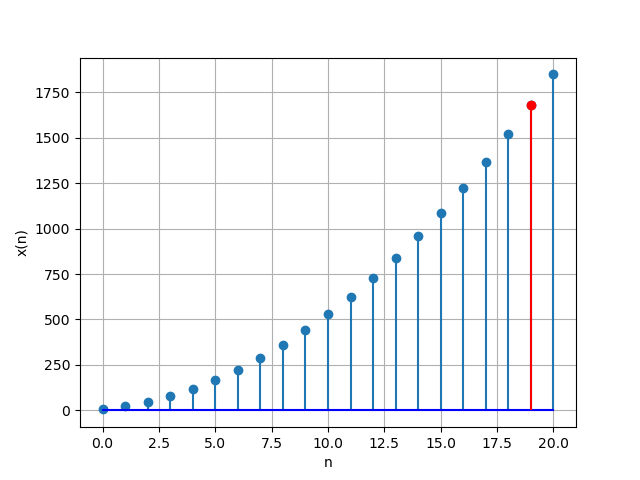
\includegraphics[width=1\columnwidth]{graphs/digital2_graph.png}
    
	\label{fig:11.9.5.22.1}
\end{figure}


\end{document}
